\PassOptionsToPackage{hyperfootnotes=false}{hyperref}
\documentclass{beamer}
\usefonttheme{professionalfonts}
%\usetheme{Rochester}
%\usetheme{AnnArbor}
\usetheme{Szeged}
\useoutertheme{infolines}
\usecolortheme{dolphin}
\usepackage{graphicx}
\usepackage{booktabs}
% \usepackage[english]{babel}
\usepackage{multicol}
\usepackage{color}
\usepackage{xcolor}
%\usepackage{smartdiagram}


%\definecolor{carmine}{rgb}{0.59, 0.0, 0.09}
\usepackage{amsmath} 

\usepackage{graphicx}
\usepackage{tikz}
\usetikzlibrary{shapes.callouts}
\usepackage{multirow}

\usepackage[utf8]{inputenc}

\usepackage{enumerate}
\usepackage[shortlabels]{enumitem}
\usepackage{amsmath,amsthm,amssymb,amsfonts,mathrsfs,latexsym,stmaryrd}
\usepackage{tcolorbox}

\usepackage{color} 
\usepackage{amssymb, amsmath, amsbsy}
\usepackage{adjustbox,lipsum}
\usepackage{placeins}

\usepackage{textpos}
\usepackage{wrapfig}
\usepackage[spanish, es-tabla]{babel}

\usepackage{caption}
\setlength{\parindent}{0pt}

\usepackage{url}
\usepackage{float}
\usepackage{tikz}
\usetikzlibrary{patterns}


\title[ICS-162]{Econometría ICS-294\\ \small{Clase 12: Propiedades asintóticas  }}

\author{Francisco Alfaro Medina}
\institute[USM]
{Universidad Técnica Federico Santa María\\ % Your institution for the title page
	\medskip
	\textit{} % Your email address
	
}
\logo{

\includegraphics[width=1cm]{Logo.png}
}
\date{}
\newcommand\Fontvi{\fontsize{9}{7.2}\selectfont}
\DeclareMathOperator{\plim}{plim}
\begin{document}

    
% Diapositiva 1: Portada
\begin{frame}
	\titlepage % Print the title page as the first slide


\end{frame}
%%%%%%%%%%%%%%%%%%%%%%%%%%%%%%%%%%%%%%%%%%%%%%%%%%%%%%%%%%%%%%%%%%%%%%%%%%%





% Diapositiva 2: Introducción
\begin{frame}{Introducción}
    \textbf{Pregunta clave:} ¿Cómo se comporta el estimador de MCO cuando el tamaño de la muestra crece indefinidamente? 
    \begin{itemize}
        \item El análisis asintótico nos permite estudiar el comportamiento del estimador en muestras grandes.
        \item Es útil para justificar inferencias cuando la normalidad exacta de los errores no se cumple.
    \end{itemize}
\end{frame}

\begin{frame}
\frametitle{Muestras finitas vs. muestras grandes}
\begin{itemize}
    \item Propiedades de muestras finitas: válidas para cualquier \(n\), como la insesgadez bajo Gauss-Markov.
    \item Propiedades asintóticas: válidas cuando \(n \to \infty\).
    \item Nos interesa estudiar el comportamiento de los estimadores cuando el tamaño de la muestra crece.
\end{itemize}
\end{frame}

\begin{frame}
\frametitle{Supuestos para la consistencia de MCO}
\begin{itemize}
\item 1) Linealidad en los parámetros.
    \item 2) Muestreo aleatorio.
    \item 3) No hay multicolinealidad perfecta. 
    \item 4) Exogeneidad: $E[u | x_1, x_2, x_3, ..., x_k] = 0$
    
\end{itemize}

Estos supuestos son los mismos del insesgamiento. 

No asumimos que la distribución de los u es normal.
\end{frame}

\begin{frame}{Un supuesto 4': exogeneidad débil}
\begin{itemize}
\item Para la \textbf{consistencia} basta con
$$E(x_i' u_i) = 0 \quad \text{(no correlación / exogeneidad débil)}$$

\item Una manera de caracterizar el supuesto de media condicional cero, $E(u|x_1, ..., x_k)=0$  es
que ninguna {\color{blue}función } de las variables explicativas está correlacionada con u. El supuesto 4'
sólo requiere que ninguna $x_j$ esté correlacionada con u.
\item Consecuencia práctica: la \textbf{omisión de variables relevantes} correlacionadas con los regresores incluidos genera \textbf{inconsistencia} (no solo sesgo), y ese sesgo asintótico \emph{no desaparece} al aumentar $n$.
\end{itemize}
\end{frame}
\begin{frame}
\frametitle{¿Qué es la consistencia?}
\begin{block}
{Un estimador es \textbf{consistente} si:} al aumentar el tamaño de la muestra, el estimador se aproxima al valor verdadero del parámetro:
\[
\hat{\beta}_j^n \xrightarrow{p} \beta_j
\]
\end{block}
\begin{itemize}
    \item En términos probabilísticos: su distribución se concentra en torno al parámetro. 
    \item A medida que el tamaño de la muestra aumenta ($n\rightarrow \infty$), la probabilidad de que el estimador est\'e muy cerca del parámetro se aproxima a 1. Es decir, los valores del estimador
  se agrupan cada vez más cerca del valor del parámetro conforme n crece.

    \item 
    {\color{blue} $Prob(|\hat{\beta}_j^n-\beta_j|>\epsilon)\rightarrow 0$ cuando $n\rightarrow \infty \quad \forall \epsilon$ } 
    
    Se escribe usando la notación \textbf{plim}: \( \plim \hat{\beta}_j^n = \beta_j \)
\end{itemize}
\end{frame}

\begin{frame}{Consistencia}
   
\begin{figure}
        \centering
        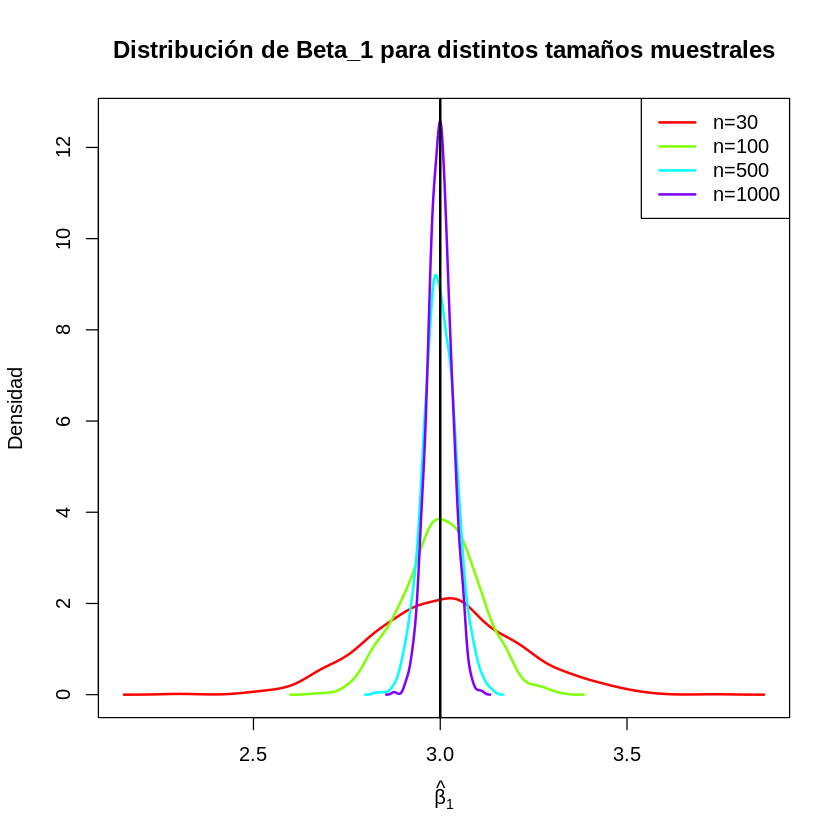
\includegraphics[width=0.7\linewidth]{Graficos Betas.png}
    \end{figure}

 
\end{frame}



% \begin{frame}{Consistencia }

% La consistencia implica
% realizar un experimento para saber lo que ocurre a medida que el tamaño de la muestra
% aumenta, mientras, al mismo tiempo, se obtienen numerosas muestras aleatorias para cada tamaño
% de muestra. Si el obtener cada vez más datos no lleva a acercarse al valor del parámetro de
% interés, entonces el procedimiento de estimación que se está usando no es adecuado.
    
% \end{frame}

% \begin{frame}{Incosistencia o sesgo asintótico}

% Ejemplo: regresión lineal simple 
%     $$plim \hat{\beta}_1 - \beta_1 =Cov(x_1, u)/Var(x_1).$$
% \end{frame}


\section{Normalidad asintótica}

\begin{frame}{Distribución normal asintótica}
\begin{definition}
Una secuencia de variables aleatorias $\{Z_n\}$ tiene una \textbf{distribución normal estándar asintótica} si para todo $z$:
$$P(Z_n \le z) \to \Phi(z) \quad \text{cuando } n \to \infty,$$
donde $\Phi(\cdot)$ es la función de distribución acumulada normal estándar. Se escribe
$$Z_n \; \dot\sim \; \text{Normal}(0,1).$$
\end{definition}
\begin{itemize}
\item Base del \textbf{Teorema Central del Límite (TCL)}: la suma (estandarizada) de v.a.i.i.d. converge a una normal, sin importar la distribución original.
\end{itemize}
\end{frame}

\begin{frame}{Normalidad asintótica de MCO }
Bajo los supuestos de Gauss-Markov (sin requerir normalidad de $u$):
$$\sqrt{n}(\hat\beta_j - \beta_j) \;\dot\sim\; \text{Normal}(0, \sigma^2 a_j^{-2})$$

En notación matricial:
$$\sqrt{n}(\hat\beta - \beta) \;\dot\sim\; \text{Normal}\big(0,\; \sigma^2 A^{-1}\big), \qquad A = E(x_i'x_i)$$

\textbf{Interpretación:} para $n$ suficientemente grande, $\hat\beta$ se distribuye \textbf{aproximadamente} normal, aun si $u$ no es normal.
\end{frame}

\begin{frame}{Idea de la demostración (caso simple)}
Se puede escribir:
$$\sqrt{n}(\hat\beta_1 - \beta_1) = (1/s_x^2)\, n^{-1/2}\sum_{i=1}^n (x_i - \bar x)u_i$$
\begin{enumerate}
\item Por LGN: $s_x^2 \xrightarrow{p} \sigma_x^2 = \text{Var}(x)$
\item $\{(x_i-\mu)u_i\}$ es i.i.d., media 0, varianza $\sigma^2\sigma_x^2$ (bajo homocedasticidad)
\item Por el \textbf{TCL}: $n^{-1/2}\sum_i (x_i-\mu)u_i \;\dot\sim\; \text{Normal}(0,\sigma^2\sigma_x^2)$
\item El término $(\mu-\bar x)\,n^{-1/2}\sum_i u_i \xrightarrow{p} 0$ (no afecta la distribución límite)
\end{enumerate}
$$\Rightarrow \sqrt{n}(\hat\beta_1-\beta_1) \;\dot\sim\; \text{Normal}(0, \sigma^2/\sigma_x^2)$$
\end{frame}

\begin{frame}{Consecuencias prácticas}
\begin{itemize}
\item Los estadísticos $t$ y $F$ tienen distribuciones \textbf{asintóticamente} $t$ / $\chi^2$, incluso sin normalidad de $u$.
\item Justifica el uso de inferencia estándar (IC, valores-$p$) en \textbf{muestras grandes}, aun si los errores no son normales.
\item El \textbf{Multiplicador de Lagrange (LM)} y el \textbf{estadístico de Wald} se basan en estos mismos resultados de convergencia.
\item Con heterocedasticidad, se reemplaza $\sigma^2 A^{-1}$ por una matriz de varianza-covarianza \textbf{robusta}:
$$\widehat{\text{Avar}}(\hat\beta) = (X'X)^{-1}\left(\sum_i \hat u_i^2\, x_i'x_i\right)(X'X)^{-1}$$
\end{itemize}
\end{frame}

% ================= SECCIÓN 4 =================
\section{Eficiencia asintótica}

\begin{frame}{Eficiencia asintótica de MCO (Teorema 5.3)}
\begin{itemize}
\item Bajo los supuestos de Gauss-Markov \textbf{más} homocedasticidad, MCO no solo es MELI (Gauss-Markov) en muestra finita.
\item Es también \textbf{asintóticamente eficiente} entre una clase amplia de estimadores (no solo lineales) que son consistentes bajo los mismos supuestos.
\item Compara la matriz de varianza-covarianza asintótica de MCO con la de cualquier otro estimador consistente y asintóticamente normal: MCO tiene la menor varianza asintótica.
\end{itemize}
\end{frame}

% ================= SECCIÓN 5 =================
\section{Síntesis}

\begin{frame}{Resumen: muestra finita vs.\ asintótica}
\begin{table}
\centering
\small
\begin{tabular}{lll}
\toprule
& \textbf{Muestra finita} & \textbf{Asintótico} \\
\midrule
Propiedad & Insesgamiento & Consistencia \\
Requiere normalidad & Sí (para $t$, $F$ exactas) & No \\
Supuesto clave & $E(u\mid x) = 0$ & $E(x'u) = 0$ \\
Herramienta & Álgebra exacta & LGN + TCL \\
Resultado & $\hat\beta \sim \text{Normal exacta}$ & $\sqrt{n}(\hat\beta-\beta) \dot\sim \text{Normal}$ \\
\bottomrule
\end{tabular}
\end{table}
\end{frame}

\begin{frame}{Puntos clave para recordar}
\begin{enumerate}
\item \textbf{Consistencia} $\neq$ insesgamiento: son propiedades distintas.
\item La \textbf{LGN} da consistencia; el \textbf{TCL} da normalidad asintótica.
\item MCO es consistente bajo supuestos \textbf{más débiles} que los necesarios para el insesgamiento.
\item La normalidad asintótica \textbf{no requiere} que $u$ sea normal — solo tamaño de muestra grande.
\item Estos resultados justifican la inferencia estándar (t, F, IC) en la práctica aplicada.
\end{enumerate}
\end{frame}

\begin{frame}{Normalidad Asintótica}

    
    \begin{equation}
         \hat{\beta}  \xrightarrow{d} N(\beta, \Sigma)
    \end{equation}
    donde $\Sigma = \sigma^2 (X'X)^{-1}$.

 {\color{blue} La convergencia en distribución   se debe al Teorema Central del Límite.}
  
    \textbf{Implicaciones:}
    \begin{itemize}
        \item Permite construir intervalos de confianza asintóticos.
        \item Justifica la inferencia estadística en muestras grandes aun cuando no se cumpla la normalidad de los errores.
    \end{itemize}
\end{frame}



 
% Diapositiva 6: Eficiencia Asintótica
\begin{frame}{Eficiencia Asintótica}
    \textbf{Definición:} Un estimador es asintóticamente eficiente si minimiza la varianza dentro de la clase de estimadores consistentes y asintóticamente normales.
    \begin{itemize}
        \item Bajo homocedasticidad, MCO es eficiente (Gauss-Markov).
        \item Bajo heterocedasticidad, MCO sigue siendo consistente, pero no eficiente (no se soluciona con muestra grande).
    \end{itemize}
\end{frame}

\begin{frame}
\frametitle{Importancia práctica}
\begin{itemize}
    \item En la práctica, siempre usamos muestras finitas.
    \item La consistencia indica que con suficientes datos, podemos acercarnos al valor verdadero.
    \item Granger (Nobel Economía 2003): \textit{“Si usted no puede obtener un resultado correcto a medida que \(n\) tiende a infinito, es mejor que se dedique a otra cosa.”}
\end{itemize}
\end{frame}

% \begin{frame}{Aplicación en R}
%     \textbf{Ejemplo: Verificación de consistencia}
%     \begin{verbatim}
%     set.seed(123)\\
%     n <- 1000\\
%     x <- rnorm(n)\\
%     u <- rnorm(n)\\
%     y <- 2 + 3*x + u\\
%     modelo <- lm(y ~ x)\\
%     summary(modelo)
%     \end{verbatim}
%     A medida que $n$ aumenta, el coeficiente estimado de $x$ se acerca a 3.
% \end{frame}

\begin{frame}{Aplicación en R: Bucle}
\href{https://colab.research.google.com/drive/1sgiL5ubKRmtMeEIaTwql5VA4dO5qxoNL?usp=sharing}{\beamergotobutton{Colab}}

\begin{figure}
        \centering
        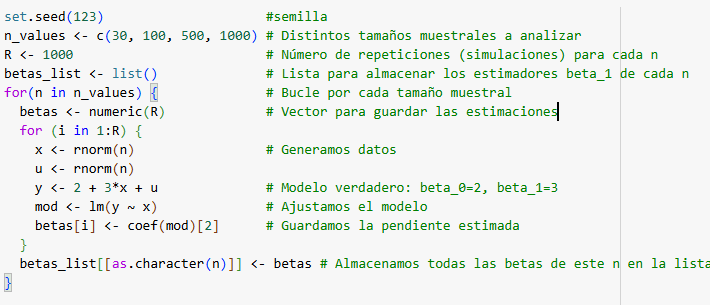
\includegraphics[width=1\linewidth]{codigoRconsistencia.png}
    \end{figure}
\end{frame}

\end{document}